\chapter{Introduction} \label{chap:introduction}

\begin{quote}
    \textit{Une intelligence qui, pour un instant donné, connaîtrait toutes les forces dont la nature est animée, et la situation respective des êtres qui la composent, si d'ailleurs elle était assez vaste pour soumettre ces données à l'analyse, embrasserait dans la même formule les mouvements des plus grands corps de l'univers et ceux du plus léger atome; rien ne serait incertain pour elle, et l'avenir, comme le passé, serait présent à ses yeux.}

    \begin{flushright}
        --- Pierre-Simon Laplace (1840) \nocite{laplace1840essai}
    \end{flushright}
\end{quote}

\vspace{1em}

Laplace's demon is a hypothetical superintelligent being that knows everything about the state of our universe, from the largest star to the smallest particle, at a single moment in time. One can imagine that the demon possesses a kind of photograph of our universe, recording not just light from one point of view, but all physical properties of all objects in all directions. Then, under the assumption that our universe is a colossal deterministic machine, nothing from ancient past to distant future is uncertain for the demon. For us, mortal humans, the picture is very different. First, we are not superintelligent. We are limited by the power of our brains and, since 1945, computers. Even if we had access to as much information as Laplace's demon, we would not be able to process it on a human timescale. Second, unlike the demon, we don't know the machinery behind our universe. Through the scientific method, we make, falsify, and replace models, but they remain incomplete.\sidenote{\textit{All models are wrong,\\some are useful.}\\[1ex] --- George Box (1976)} In fact, to this day, it is still debated whether our universe is inherently deterministic or stochastic~\cite{bell1964einstein, genovese2005research, larsson2014loopholes}. If it is stochastic, no amount of information would be enough to predict the future with certainty. Third, and perhaps most importantly, we are rarely certain about the state of a system, let alone of our universe. Our instruments, which enable us to probe systems and gather observations, are never perfect and always carry some level of measurement error. Even if we could develop more precise instruments, Heisenberg's uncertainty principle~\cite{heisenberg1927ueber} states that there is a fundamental limit to the precision with which some physical properties, such as position and momentum, can be known simultaneously. All these limitations make human beings inherently uncertain.\sidenote{\vspace{-2em}\textit{Le doute n'est pas\\un état bien agréable,\\mais l'assurance est\\un état ridicule.}\\[1ex] --- Voltaire (1770)}

Despite our doubts, we are and have been obsessed with predicting the future for millennia. From the Babylonians and Mayans to the Chinese and Greeks, we have tried to predict the movements of planets, the changes in weather, the apparition of natural disasters, and much more. Our ancestors, who were more vulnerable to their environment than we are today, predicted out of necessity: they had to protect, feed, and shelter their families. Unfortunately, while ancient astronomers made remarkably acute predictions of planetary and stellar motions, weather forecasting remained wildly speculative for centuries. It is only by the end of the Renaissance that the first instruments to measure temperature and atmospheric pressure, the thermometer and barometer, were invented by Italian physicists Galileo Galilei and Evangelista Torricelli. These early instruments, and those that followed, enabled individuals to make and record surface measurements across the globe. The later emergence of telegraph networks, during the nineteenth century, made it possible to share and compile observations routinely. Crude weather maps were drawn and surface wind patterns started to be identified and studied. At the turn of the twentieth century, \textcite{abbe1901physical} and \textcite{bjerknes2009problem} proposed that the laws of physics could be used to model the atmospheric dynamics and forecast the weather. This proposition was audacious at that time, as there were few routine observations of the atmosphere, limited understanding of meteorological mechanisms, and no computers. Since, there has been continued investment and advances in the observational, theoretical and computational aspects of geosciences, enabling ever more reliable weather forecasts. Meteorological instruments now include polar-orbiting and geostationary satellites, ocean buoys, cloud radars, and surface weather stations, among many others. This network of instruments, illustrated in Figure \ref{fig:gos}, is known as the Global Observing System~\cite{worldmeteorologicalorganization2020observation} and is in constant expansion.

\begin{figure}[b]
    \centering
    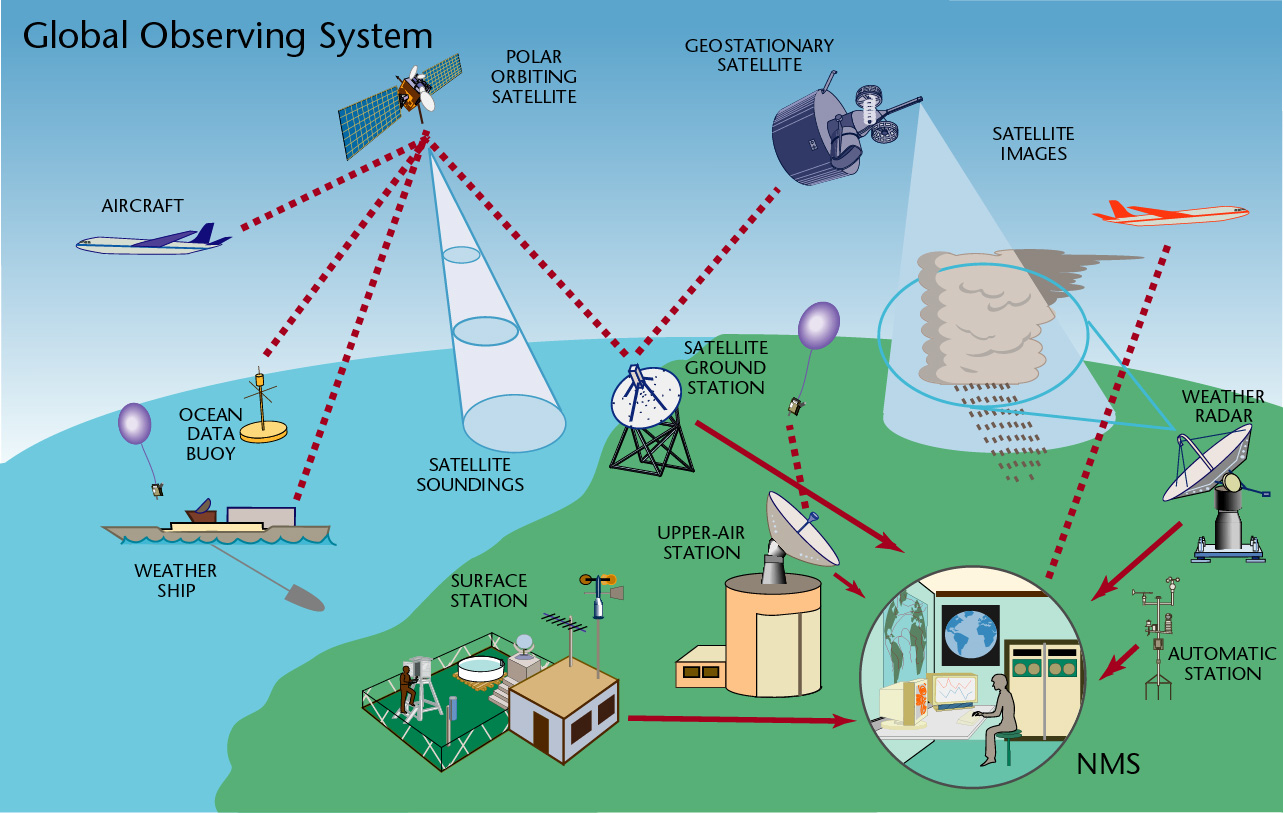
\includegraphics[width=0.66\textwidth]{./figures/gos.jpg}
    \caption{Illustration of the components of the Global Observing System (GOS) by the \textcite{worldmeteorologicalorganization2020observation}.}
    \label{fig:gos}
\end{figure}

However, better and higher-resolution instruments imply greater sensitivity to physical and chemical processes in the oceans and atmosphere, which in turn increases the complexity of the theoretical models required to interpret their measurements. The growing number of instruments also introduces new challenges in terms of quantity of collected data. Most notably, the use of satellite data has increased exponentially over the last two decades, becoming the largest contributor to forecast quality~\cite{jeppesen2020ecmwfs} and pushing current numerical weather prediction (NWP) methods to their limits. In fact, an overwhelming majority (90 to \qty{95}{\percent}) of the available satellite data is unexploited by operational NWP centers~\cite{bauer2015quiet}, including satellite channels in the visible and infrared spectrum, despite providing a wealth of information on atmospheric clouds~\cite{scheck2020assimilating, kugler2023potential}. These observations stand largely unassimilated because (a) efficient models of their measurement processes are still lacking, and (b) scaling current pipelines to ingest their volume remains computationally intractable.

Undeterred by these challenges, meteorologists across the globe continue their work towards more accurate weather prediction, for its impact is among the greatest of any field in the physical sciences~\cite{bauer2015quiet}. However, many now argue that, instead of investing solely in new instruments and increasingly sophisticated models, NWP should adopt a new computational paradigm; one that is more efficient, takes full advantage of modern hardware, and learns from the vast amounts of available data. This is where machine learning and, more specifically, deep learning come into play. Amid this abundance of data, where experts struggle to extract patterns and leverage domain knowledge, machines can learn efficient models automatically.\sidenote{\vspace{-4em}\textit{Machines take me by surprise with great frequency.}\\[1ex] --- Alan Turing (1950) \nocite{turing1950computing}} Over the past decade, this has proven true for an increasingly broad spectrum of tasks, including language modeling~\cite{vaswani2017attention, devlin2019bert, brown2020language}, voice processing~\cite{oord2016wavenet, radford2022robust, goel2022its}, image synthesis~\cite{zhu2017unpaired, karras2019stylebased, rombach2022highresolution}, autonomous agents~\cite{mnih2015humanlevel, silver2017mastering, baker2020emergent, andrychowicz2020learning, wei2022chainofthought}, and numerous scientific applications~\cite{jumper2021highly, rolnick2022tackling, degrave2022magnetic, merchant2023scaling, pfau2024accurate, manduchi2024leveraging}. Following this success, a wave of research has sought to enhance or replace NWP components with deep learning models~\cite{ravuri2021skilful, dueben2021machine, mack2020attentionbased, brajard2020combining, brajard2021combining, arcucci2021deep, fablet2021learning, frerix2021variational, buizza2022data, yeung2022physicsinformed, andrychowicz2023deep, lam2023learning}, some of which have already been integrated into operational pipelines~\cite{lang2024aifs, lentze2025ecmwfs}.

Still, unless one is akin to Laplace's demon, prediction remains fundamentally riddled with uncertainty. While there has been a long history of work to integrate deep learning models in the natural sciences, it is only recently that practitioners have started using deep \emph{probabilistic} models. These models explicitly take uncertainty into account and learn the non-deterministic relationships between the quantities of interest. Among the first deep probabilistic models were probability density estimators, including density ratio estimators \cite{tu2007learning, sugiyama2012density, gutmann2012noisecontrastive, cranmer2016approximating, cranmer2016experiments, menon2016linking, stoye2018likelihoodfree, belghazi2018mutual, durkan2020contrastive, rhodes2020telescoping, brehmer2020mining, hermans2020likelihoodfree, miller2021truncated, rozet2021arbitrary, miller2022contrastive, delaunoy2022reliable, choi2022density} and normalizing flows \cite{tabak2013family, dinh2014nice, rezende2015variational, dinh2016density, papamakarios2017masked, huang2018neural, wehenkel2019unconstrained, durkan2019neural, papamakarios2021normalizing}. One area where density estimators became the gold standard is simulation-based inference~\cite{cranmer2020frontier}, which is now recognized as a valuable extension to the statistical toolbox used in particle physics~\cite{atlascollaboration2025implementation}.

Unfortunately, density estimators have classically been restricted to low-dimensional settings, making their application to high-dimensional problems, such as those encountered in earth sciences, challenging. Furthermore, while estimating the probability density has many use cases, drawing samples from a target distribution is often the objective of probabilistic approaches. In response to these needs, a new class of deep probabilistic models has emerged, that can efficiently generate samples from high-dimensional distributions. These \emph{generative} models notably include variational auto-encoders \cite{kingma2013autoencoding, kingma2019introduction}, generative adversarial networks \cite{goodfellow2014generative}, and, most recently, diffusion models \cite{sohl-dickstein2015deep, ho2020denoising}, also known as score-based generative models \cite{song2019generative, song2021scorebased}, flow models \cite{liu2023flow, lipman2023flow}, or stochastic interpolants \cite{albergo2023stochastic}. Since their introduction, generative models have received widespread adoption in the context of image, video, and audio synthesis, and their success is now spreading to all areas of natural sciences.

\section{Research Question}

Motivated by the recent wave of research to solve scientific problems with deep probabilistic models, and the remaining obstacles to tackle high-dimensional settings, this thesis focuses on developing and applying generative models to large-scale inference problems in physics, particularly in systems whose state evolves through time, known as dynamical systems.\sidenote{\vspace{-2em}\textit{I will not define time, space, place and motion, as being well known to all.}\\[1ex] --- Isaac Newton (1687) \nocite{newton1687philosophiae}} The rapid evolution of deep learning and the modern abundance of scientific data make this objective not only timely, but a unique opportunity for technological progress.

In pursuit of this objective, this thesis explores several aspects of probabilistic modeling and dynamical systems, including state estimation, forecasting, reduced-order modeling, and learning from corrupted observations. Although motivated and developed in the context of scientific applications, the methodological contributions extend to the broader field of generative modeling.

\section{Outline}

Immediately following this introduction, we present the main contributions of this thesis, which are based on a series of peer-reviewed publications. We choose not to include an original primer on dynamical systems or deep probabilistic modeling as part of this dissertation. These topics are thoroughly covered in the literature through numerous books and reviews, and our own attempts could not match their clarity and completeness. We notably recommend two excellent reviews by \textcite{carrassi2018data} and \textcite{lai2025principles} on data assimilation and diffusion models, respectively. The background concepts and relevant literature are nevertheless discussed within the respective chapter of each contribution.

Opening the scientific part of this dissertation, Chapter \ref{chap:sda} investigates the application of diffusion models~\cite{sohl-dickstein2015deep, ho2020denoising} to the problem of state estimation in dynamical systems. This work establishes diffusion models as a promising and versatile alternative to classical data assimilation \cite{ledimet1986variational, hamill2006ensemblebased, evensen2009data, carrassi2018data, ecmwf2020ifs} methods. Chapter \ref{chap:sda-2lqg} further demonstrates that the method presented in Chapter \ref{chap:sda}, named score-based data assimilation (SDA), scales effectively to near-operational-scale systems. However, the data SDA relies on for training -- fully observed state sequences -- is rarely accessible. In practice, only incomplete and noisy observations of the states are available, especially in earth and space sciences where the systems of interest can only be probed superficially. Chapter \ref{chap:diem} addresses this limitation in the broader context of learning a prior distribution parameterized by a diffusion model when only partial and noisy observations are available. The proposed method is an adaptation of the expectation-maximization \cite{hartley1958maximum, dempster1977maximum, wu1983convergence, mclachlan2007em, balakrishnan2017statistical} algorithm tailored to diffusion models. Another limitation of SDA is its computational cost, which becomes prohibitive for long trajectories and high-dimensional states. In the context of image and video generation, this computational obstacle has been mitigated by generating in the latent space of an autoencoder rather than in pixel space. In Chapter \ref{chap:lola}, we investigate whether a similar strategy can be effectively applied to the emulation of dynamical systems, and at what cost. Our results indicate that latent modeling is a promising approach; one that is not only more efficient, but can also improve accuracy compared to physics-space models. Encouraged by these findings, we combine the latent modeling approach with the SDA framework in Chapter \ref{chap:appa}, obtaining promising results on operational-scale atmospheric data assimilation tasks.

Finally, Chapter \ref{chap:discussion} reflects upon the contributions of this thesis and discusses possible future developments in deep probabilistic modeling and its applications to dynamical systems.

\section{Publications}

The scientific content of this dissertation is exclusively borrowed from the following peer-reviewed publications, for which I played the role of lead author or project instigator.

\begin{itemize}[leftmargin=1em]
    \item[] \fullcite{rozet2023scorebased}.
    \item[] \fullcite{rozet2023scorebaseda}.
    \item[] \fullcite{rozet2024learning}.
    \item[] \fullcite{rozet2025lost}.
    \item[] \fullcite{andry2025appa}.
\end{itemize}

Throughout the pursuit of my degree, I also had the chance to take part and contribute to fruitful collaborations. The following list of publications, which are not featured in this thesis, stemmed from these collaborations.

\begin{itemize}[leftmargin=1em]
    \item[] \fullcite{hermans2022trust}.
    \item[] \fullcite{delaunoy2022reliable}.
    \item[] \fullcite{vasist2023neural}.
    \item[] \fullcite{ohana2024well}.
    \item[] \fullcite{savary2025trainingfree}.
    \item[] \fullcite{morel2025predicting}.
    \item[] \fullcite{mccabe2025walrus}.
\end{itemize}

Finally, over the past years, I have devoted a significant part of my time to free and open-source software. I consider the following Python packages, which I created and maintained during my degree, to be among its contributions.

\begin{itemize}[leftmargin=1em]
    \item[] \fullcite{rozet2021lampe}.\\ \url{https://pypi.org/project/lampe}
    \item[] \fullcite{rozet2022zuko}.\\ \url{https://pypi.org/project/zuko}
    \item[] \fullcite{rozet2024azula}.\\ \url{https://pypi.org/project/azula}
\end{itemize}

\clearpage
\section*{References}

\printbibliography[heading=none]
